\documentclass{llncs}

\usepackage{amsmath}
\usepackage{graphicx}
\usepackage{url}
\usepackage{booktabs}
\usepackage{tabularx}
\usepackage{xcolor}
\usepackage{tikz}
\usetikzlibrary{arrows.meta,positioning}
\providecommand{\email}[1]{\texttt{#1}}
\graphicspath{{.}{figures/}}
\renewcommand{\topfraction}{0.9}
\renewcommand{\textfraction}{0.1}
\renewcommand{\floatpagefraction}{0.8}


\begin{document}

\title{Performance Analysis of Apache ZooKeeper's Write Pipeline\\
\large Software Performance Engineering --- Project Stage II}

\author{Gil Jorge (110062) \and Jo\~{a}o Palma (109242) \and Gabriel Petti Tavares (120691)}

\institute{Instituto Superior T\'{e}cnico, Universidade de Lisboa --- Group 18\\
  \email{gil.jorge@tecnico.ulisboa.pt}, \email{joaofontepalma@tecnico.ulisboa.pt},
  \email{gabriel.p.tavares@tecnico.ulisboa.pt}}

\maketitle

\begin{abstract}
ZooKeeper answers reads at any server but sends every write through one leader and a quorum. We study the cost of
that write pipeline on Google Compute Engine with a $2^{6-1}$ factorial experiment (two replicates), one replicated
Universal Scalability Law curve and five eBPF probes. The write ratio explains 60\% of the variation of throughput and
the number of clients 94\% of the variation of the write tail latency. Turning \texttt{fsync} off helps at light load
(+39\%) and hurts at saturation ($-17\%$). The curve needs only a contention term ($\sigma=0.039$); the disk is not where
that contention comes from, but our data do not single out one stage of the leader either. We also report a client-side
logging artifact that had distorted the Stage I fits.
\end{abstract}

\noindent\textbf{Git Commit Identifier:} \texttt{9a52eabcfe0019b8ab4ac96fb7bb2195694d70a0}

\section{Introduction}

Apache ZooKeeper is a coordination service used by Kafka, HBase and Hadoop for leader election, configuration and
locks~\cite{hunt_zookeeper,apache_zookeeper_overview}. Its replication protocol, Zab~\cite{zab_junqueira}, makes reads
and writes behave very differently: a read is answered by the server the client is connected to, while a write goes
to the leader, is logged and acknowledged by a majority and only then committed. Reads should therefore scale with the
number of servers and writes should not, and the write pipeline is where we look for the limits of scalability.

Stage I measured one laptop with Docker and fitted the Universal Scalability Law
(USL)~\cite{gunther_usl_dsconf,gunther_book}. In Stage II we (1) found and removed a client-side artifact in the Stage I
data (Section~\ref{sec:stage1}); (2) ran a fractional factorial experiment on dedicated virtual machines to rank the
factors that drive throughput and write tail latency (Sections~\ref{sec:design}--\ref{sec:factorial}); (3) fitted one
replicated USL curve and recorded ZooKeeper's per-stage timers at every load level (Section~\ref{sec:usl}); and
(4) observed the leader with eBPF (Section~\ref{sec:ebpf}).

\section{System Description}

ZooKeeper keeps a tree of small data nodes (znodes) in memory and persists every change in a transaction log. $N=2f+1$
servers elect a \emph{leader}, tolerate $f$ failures and stop accepting writes when no majority is
reachable~\cite{zab_junqueira}. Writes are linearizable; reads are sequentially consistent per session and may be
slightly stale, which is what allows a follower to answer them alone~\cite{hunt_zookeeper}. Figure~\ref{fig:pipeline}
shows both paths.

\begin{figure}[t]
  \centering
  \resizebox{\textwidth}{!}{%
  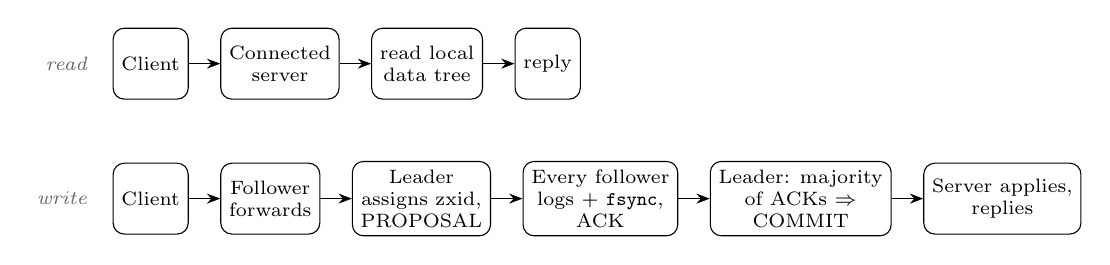
\begin{tikzpicture}[>=Stealth, node distance=4mm,
      box/.style={draw, rounded corners, font=\scriptsize, align=center, inner sep=3pt, minimum height=9mm},
      lab/.style={font=\scriptsize\itshape, text=black!60}]
    \node[box] (rc) {Client};
    \node[box, right=of rc] (rs) {Connected\\server};
    \node[box, right=of rs] (rr) {read local\\data tree};
    \node[box, right=of rr] (rd) {reply};
    \draw[->] (rc)--(rs); \draw[->] (rs)--(rr); \draw[->] (rr)--(rd);
    \node[lab, left=2mm of rc, anchor=east] {read};

    \node[box, below=8mm of rc] (wc) {Client};
    \node[box, right=of wc] (wf) {Follower\\forwards};
    \node[box, right=of wf] (wl) {Leader\\assigns zxid,\\PROPOSAL};
    \node[box, right=of wl] (wa) {Every follower\\logs + \texttt{fsync},\\ACK};
    \node[box, right=of wa] (wq) {Leader: majority\\of ACKs $\Rightarrow$\\COMMIT};
    \node[box, right=of wq] (wr) {Server applies,\\replies};
    \draw[->] (wc)--(wf); \draw[->] (wf)--(wl); \draw[->] (wl)--(wa); \draw[->] (wa)--(wq); \draw[->] (wq)--(wr);
    \node[lab, left=2mm of wc, anchor=east] {write};
  \end{tikzpicture}}
  \caption{Read and write paths in ZooKeeper.}
  \label{fig:pipeline}
\end{figure}

Inside the leader a write passes a chain of processors. Request preparation (one thread) validates it and assigns the
zxid; the log-sync stage (one thread) appends it to the log and calls \texttt{fsync}, writing every request that is queued
at that moment in one batch (group commit); the commit stage applies it once a majority has acknowledged. The followers
run the same log-sync stage before they acknowledge. A read costs one hop and no coordination; a write costs a forward,
a proposal to every follower, a log write and \texttt{fsync} on each, acknowledgments and a commit.

\section{Stage I}
\label{sec:stage1}

In Stage I the same configuration (3 servers, 20 clients, 30\% writes) gave 6{,}364 ops/s in the sweep and 14{,}832 ops/s
when we repeated it later. The jar used for the sweep bundled Logback, whose default configuration logs the ZooKeeper
client at DEBUG level: it printed about 145{,}000 lines in a 15\,s run, one per operation, and all client threads
waited on the console. The fix is a one-line Logback configuration, and the runner now aborts any run in which the client
prints more than a few lines. This changes the Stage I conclusion. The fits had given the same contention coefficient
($\approx0.23$) for 1, 3 and 5 servers, which we read as server-side contention unrelated to Zab; a bottleneck in the
client also produces a coefficient that does not depend on the number of servers. With the quiet client the coefficient
was 0.025, 0.088 and 0.112 for 1, 3 and 5 servers. In the same comparison, repetitions of one variant on the laptop
differed by up to a factor of two, and the sweep had one run per point in increasing order of load. Stage II therefore uses
separate machines for client and servers, replicates and a randomized order. The Stage I experiments that we did not
repeat on the new testbed (YCSB, leader failover, injected network delay) are summarized in Appendix~\ref{app:stage1}
and are not used for any conclusion of this report.

\section{Testbed and Methodology}
\label{sec:method}

\paragraph{Deployment.} All Stage II runs use Google Compute Engine in one zone (europe-west1-b). The load generator has
its own n2-standard-8 machine (8 vCPUs, 32\,GB); every ZooKeeper server has an n2-standard-2 (2 vCPUs, 8\,GB). All run
Debian~12 (kernel 6.1) and OpenJDK~17. ZooKeeper 3.9.3 runs natively with a 1\,GB heap. Each server has two extra 20\,GB
disks, pd-balanced and pd-ssd, formatted with ext4; the transaction log goes on one of them according to the factor
\emph{log disk}, and snapshots stay on the boot disk. Before each block of runs the servers are stopped, their data is
erased and they are restarted with the new configuration; the runner then checks on every server that the
\texttt{forceSync} flag and the log directory of the running process are the intended ones.

\paragraph{Load generator.} A Java client opens one ZooKeeper session per simulated client, spread over all servers by
the connect string. Each client is a closed loop of synchronous calls without think time: it picks one of 200 znodes
uniformly and sends a \texttt{setData} with probability equal to the write ratio, otherwise a \texttt{getData}. All
sessions connect before a barrier releases them. Operations that start in the first 5\,s are executed but not recorded,
so that the JIT compilation of client and server code and the filling of caches fall outside the measurement; we did not
measure the length of that transient separately, but every series starts with a discarded run as well. A factorial run then
measures 20\,s and a USL run 30\,s. The slowest factorial run still completed more than 30{,}000 writes, so its 99th
percentile rests on over 300 samples. Percentiles are exact (all latencies are kept and sorted). The client machine logs
its own CPU every second; it never exceeded 47\% busy, so the client was not the bottleneck.

\paragraph{ZooKeeper's per-stage timers.} The \texttt{mntr} command reports, per stage, a count and a sum: the time
a request waits for the request-preparation thread, the time in the log-sync queue and flush, the \texttt{fsync} time,
requests per \texttt{fsync} and the time from proposal to quorum acknowledgment. We take a snapshot of every server before
and after each run; the difference of the sums over the difference of the counts is the mean of that run. The timers
have 1\,ms resolution and truncate, so the \texttt{fsync} is also measured with eBPF.

\paragraph{Threats to validity.} The virtual machines share physical hosts with other tenants. Replicates and the
random order spread that noise over all treatments but do not remove it: two replicates of the same factorial run differ
by 11\% at the median and by up to 48\%. One zone means short round trips between servers. \texttt{forceSync=no} is unsafe
in production and serves only as a probe.

\section{Experimental Design}
\label{sec:design}

\paragraph{Parameters.} Table~\ref{tab:params} lists the fixed system and workload parameters; the six factors and their
levels are in Table~\ref{tab:factors}.

\begin{table}[t]
  \centering
  \caption{Fixed parameters. Defaults are those of ZooKeeper~3.9~\cite{zookeeper_admin}.}
  \label{tab:params}
  \scriptsize
  \begin{tabularx}{\linewidth}{@{}>{\raggedright\arraybackslash}X>{\raggedright\arraybackslash}X@{}}
    \toprule
    Parameter & Value \\
    \midrule
    Observers; \texttt{leaderServes} & 0; yes (default) \\
    Snapshot device (\texttt{dataDir}) & boot disk (pd-standard) \\
    \texttt{snapCount}, \texttt{preAllocSize} & 100{,}000, 64\,MB (defaults) \\
    \texttt{maxBatchSize}, \texttt{flushDelay} & 1000, 0 (defaults) \\
    \texttt{globalOutstandingLimit}, \texttt{maxClientCnxns} & 1000 (default), no limit \\
    \texttt{tickTime}, \texttt{initLimit}, \texttt{syncLimit} & 2000\,ms, 10, 5 \\
    Server JVM; versions & JDK~17, 1\,GB heap, G1; ZooKeeper 3.9.3, client 3.9.0 \\
    Operations; key space & \texttt{getData}/\texttt{setData} only; 200 znodes, uniform, new pool per run \\
    Client model; session placement & closed loop, synchronous, no think time; random server \\
    Run length & 5\,s warm-up + 20\,s (factorial) or 30\,s (USL) measured \\
    \bottomrule
  \end{tabularx}
\end{table}

\paragraph{Metrics.} The primary response is throughput (successful operations per second), the quantity the USL models.
The secondary response is the 99th-percentile write latency, because a coordination service sits on the critical path of
other systems. We do not use the mean latency as a separate response: in a closed loop without think time Little's law
gives the mean response time $R=N/X$, so it carries no information beyond throughput. Failed operations (there were none)
and the client's CPU are recorded as validity checks.

\paragraph{Factors and levels.} Each factor tests one guess about where a write spends its time (Table~\ref{tab:factors}).
We chose 10 and 160 clients from the Stage I curve, where 10 was below the knee. On the new testbed the throughput per
client at 10 clients is already about 70\% of that of a single client (Section~\ref{sec:usl}), so the low level is light
load and the high level is deep in saturation. A write ratio of 0.1 is close to the 10:1 read/write ratio cited
in~\cite{mit_6824_zookeeper}; 0.5 loads the write path. Three and five servers are the usual sizes. The payloads bracket
small metadata and configuration blobs. Persistent Disk performance depends on disk and machine size, so the two disk
types are levels of this testbed only.

\begin{table}[t]
  \centering
  \caption{Factors and levels. ``Hard'': changing it needs a rebuild of the servers.}
  \label{tab:factors}
  \scriptsize
  \begin{tabular}{@{}cllllp{4.6cm}@{}}
\toprule
& Factor & $-1$ & $+1$ & Hard & Why \\
\midrule
A & ensemble\_size & 3 & 5 & yes & quorum size: proposals and ACKs per write; the two usual production sizes \\
B & write\_ratio & 0.1 & 0.5 &  & share of requests that take the write pipeline (reads stay local) \\
C & clients & 10 & 160 &  & below the saturation knee vs well beyond it \\
D & force\_sync & yes & no & yes & removes the fsync from the write path: tests the log-sync stage \\
E & payload\_bytes & 128 & 4096 &  & bytes logged, sent to every follower and synced per write \\
F & log\_disk & pd-balanced & pd-ssd & yes & speed of the device under the fsync (dedicated log disk) \\
\bottomrule
\end{tabular}

\end{table}

\paragraph{Design.} We use the half fraction $2^{6-1}$ with $F=ABCDE$ (defining relation $I=ABCDEF$)~\cite{jain_book}. It
has resolution VI: main effects are aliased with five-factor interactions and two-factor interactions with four-factor
ones, so all six main effects and fifteen two-factor interactions are estimated from 32 runs per replicate if interactions
of order four and higher are negligible. A quarter fraction would have resolution IV and alias two-factor interactions in
pairs, which is where hypotheses H2--H4 sit. Table~\ref{tab:sign} is the sign table: the full $2^5$ table of A--E with
$F$ as the product of the other five columns. With two replicates there are 64 runs and 32 degrees of freedom for error.

\begin{table}[t]
  \centering
  \caption{Sign table of the $2^{6-1}$ design with the mean throughput of the two replicates ($\bar y$, ops/s).}
  \label{tab:sign}
  \scriptsize
  \setlength{\tabcolsep}{2.6pt}
  \begin{tabular}{@{}rccccccr@{\qquad}rccccccr@{}}
\toprule
Run & A & B & C & D & E & F & $\overline{\log_{10} y}$ & Run & A & B & C & D & E & F & $\overline{\log_{10} y}$ \\
\midrule
1 & $-$ & $-$ & $-$ & $-$ & $-$ & $-$ & 4.409 & 17 & $-$ & $-$ & $-$ & $-$ & $+$ & $+$ & 4.226 \\
2 & $+$ & $-$ & $-$ & $-$ & $-$ & $+$ & 4.402 & 18 & $+$ & $-$ & $-$ & $-$ & $+$ & $-$ & 4.227 \\
3 & $-$ & $+$ & $-$ & $-$ & $-$ & $+$ & 3.944 & 19 & $-$ & $+$ & $-$ & $-$ & $+$ & $-$ & 3.752 \\
4 & $+$ & $+$ & $-$ & $-$ & $-$ & $-$ & 3.986 & 20 & $+$ & $+$ & $-$ & $-$ & $+$ & $+$ & 3.796 \\
5 & $-$ & $-$ & $+$ & $-$ & $-$ & $+$ & 4.723 & 21 & $-$ & $-$ & $+$ & $-$ & $+$ & $-$ & 4.656 \\
6 & $+$ & $-$ & $+$ & $-$ & $-$ & $-$ & 4.902 & 22 & $+$ & $-$ & $+$ & $-$ & $+$ & $+$ & 4.731 \\
7 & $-$ & $+$ & $+$ & $-$ & $-$ & $-$ & 4.300 & 23 & $-$ & $+$ & $+$ & $-$ & $+$ & $+$ & 4.183 \\
8 & $+$ & $+$ & $+$ & $-$ & $-$ & $+$ & 4.306 & 24 & $+$ & $+$ & $+$ & $-$ & $+$ & $-$ & 4.215 \\
9 & $-$ & $-$ & $-$ & $+$ & $-$ & $+$ & 4.472 & 25 & $-$ & $-$ & $-$ & $+$ & $+$ & $-$ & 4.343 \\
10 & $+$ & $-$ & $-$ & $+$ & $-$ & $-$ & 4.511 & 26 & $+$ & $-$ & $-$ & $+$ & $+$ & $+$ & 4.415 \\
11 & $-$ & $+$ & $-$ & $+$ & $-$ & $-$ & 4.093 & 27 & $-$ & $+$ & $-$ & $+$ & $+$ & $+$ & 3.980 \\
12 & $+$ & $+$ & $-$ & $+$ & $-$ & $+$ & 4.077 & 28 & $+$ & $+$ & $-$ & $+$ & $+$ & $-$ & 3.984 \\
13 & $-$ & $-$ & $+$ & $+$ & $-$ & $-$ & 4.684 & 29 & $-$ & $-$ & $+$ & $+$ & $+$ & $+$ & 4.575 \\
14 & $+$ & $-$ & $+$ & $+$ & $-$ & $+$ & 4.775 & 30 & $+$ & $-$ & $+$ & $+$ & $+$ & $-$ & 4.597 \\
15 & $-$ & $+$ & $+$ & $+$ & $-$ & $+$ & 4.106 & 31 & $-$ & $+$ & $+$ & $+$ & $+$ & $-$ & 4.082 \\
16 & $+$ & $+$ & $+$ & $+$ & $-$ & $-$ & 4.360 & 32 & $+$ & $+$ & $+$ & $+$ & $+$ & $+$ & 4.177 \\
\midrule
$q$ & +0.029 & -0.228 & +0.149 & +0.015 & -0.066 & -0.007 & 4.312 &  &  &  &  &  &  &  &  \\
\bottomrule
\end{tabular}

\end{table}

\paragraph{Restricted randomization.} A, D and F need a rebuild of the servers. Runs sharing their levels form a block
(eight blocks of four runs per replicate, 16 rebuilds in total). The block order is randomized in each replicate, and so is
the run order inside each block. The plan was generated with a fixed seed before the first run. This is a split-plot
structure: the block, not the run, is the experimental unit of A, D and F. Our main analysis tests all effects against the
pooled run error; for A, D and F we repeat the test against a whole-plot error estimated from the 16 block means
(replicate $\times$ treatment, 7 degrees of freedom).

\paragraph{Analysis.} With $s_{ij}$ the sign of run $i$ for effect $j$, $\bar y_i$ the mean of the $r=2$ replicates and
$n=32$,
\begin{equation}
  q_j=\frac1n\sum_{i} s_{ij}\,\bar y_i,\quad
  SS_j=n r q_j^2,
\end{equation}
\begin{equation}
  s_e^2=\frac{\sum_{i,k}(y_{ik}-\bar y_i)^2}{n(r-1)},\quad
  q_j \pm t_{[0.975;\,n(r-1)]}\frac{s_e}{\sqrt{n r}},
\end{equation}
and effect $j$ explains $100\,SS_j/SST$ percent of the variation. Testing 31 effects at 95\% would produce about two
false positives, so we rank effects by their share of the variation. When $y_{\max}/y_{\min}>10$ we analyse
$\log_{10}y$; residual plots are in Appendix~\ref{app:residuals}. We tested the analysis code on synthetic data with known
effects before using it.

\paragraph{Hypotheses.} Written before the runs:
\textbf{H1}: turning \texttt{fsync} off (D) raises throughput and lowers the write p99.
\textbf{H2}: that benefit grows with the write ratio (B$\times$D), since reads never touch the log.
\textbf{H3}: a faster log disk (F) helps only while \texttt{fsync} is on (D$\times$F).
\textbf{H4}: five servers (A) lower throughput and raise the write p99, mostly through writes (A$\times$B).
\textbf{H5}: the number of clients (C) has the largest main effect on throughput.

\section{Results}

\subsection{Factorial experiment}
\label{sec:factorial}

All 64 runs completed without errors. Throughput ranged from 5{,}335 to 81{,}088 ops/s and the write p99 from 1.2 to
61\,ms. Both ratios exceed 10, and the residuals of the additive model widen with the predicted value, so both responses
are analysed on $\log_{10}$, where the residuals look homogeneous and roughly normal (Fig.~\ref{fig:residuals}). Effects
are then multiplicative factors (Table~\ref{tab:effects}). The error explains 2.1\% (throughput) and 1.3\% (p99) of the
variation. That is a share of the total, and it is small because the factors change throughput up to fifteen-fold; in
absolute terms the replicates still differ by about 11\%.

\begin{table}[t]
  \centering
  \caption{Largest effects ($\log_{10}$ model): $q$, the factor ($\times$) from the low to the high level, the 95\%
    interval of $q$ and the share of the variation (\%). $^\dagger$: interval includes zero.}
  \label{tab:effects}
  \scriptsize
  \setlength{\tabcolsep}{3pt}
  \begin{tabular}{@{}lrrrrrr@{}}
\toprule
 & \multicolumn{3}{c}{throughput (ops/s), $\log_{10}$} & \multicolumn{3}{c}{write p99 (ms), $\log_{10}$} \\
\cmidrule(lr){2-4}\cmidrule(lr){5-7}
Effect & $q$ ($\times$) & 95\% CI & \% & $q$ ($\times$) & 95\% CI & \% \\
\midrule
C & 0.149 ($\times$1.98) & [0.133, 0.164] & 25.6 & 0.534 ($\times$11.68) & [0.511, 0.556] & 93.7 \\
B & -0.228 ($\times$0.35) & [-0.244, -0.213] & 60.3 & 0.041 ($\times$1.21) & [0.018, 0.064] & 0.6 \\
E & -0.066 ($\times$0.74) & [-0.081, -0.051] & 5.0 & 0.061 ($\times$1.32) & [0.038, 0.084] & 1.2 \\
C$\times$D & -0.056 ($\times$0.77) & [-0.071, -0.041] & 3.6 & 0.059 ($\times$1.31) & [0.036, 0.081] & 1.1 \\
A & 0.029 ($\times$1.14) & [0.014, 0.044] & 1.0 & 0.021 ($\times$1.10)$^\dagger$ & [-0.001, 0.044] & 0.2 \\
D & 0.015 ($\times$1.07)$^\dagger$ & [-0.001, 0.030] & 0.3 & -0.042 ($\times$0.82) & [-0.065, -0.019] & 0.6 \\
E$\times$F & 0.021 ($\times$1.10) & [0.006, 0.036] & 0.5 & -0.004 ($\times$0.98)$^\dagger$ & [-0.027, 0.018] & 0.0 \\
A$\times$B & 0.000 ($\times$1.00)$^\dagger$ & [-0.016, 0.015] & 0.0 & -0.034 ($\times$0.85) & [-0.057, -0.012] & 0.4 \\
A$\times$C & 0.018 ($\times$1.09) & [0.003, 0.033] & 0.4 & 0.010 ($\times$1.05)$^\dagger$ & [-0.013, 0.033] & 0.0 \\
B$\times$C & -0.016 ($\times$0.93) & [-0.032, -0.001] & 0.3 & -0.020 ($\times$0.91)$^\dagger$ & [-0.043, 0.003] & 0.1 \\
B$\times$E & 0.003 ($\times$1.01)$^\dagger$ & [-0.012, 0.019] & 0.0 & -0.022 ($\times$0.90)$^\dagger$ & [-0.045, 0.000] & 0.2 \\
\bottomrule
\end{tabular}

\end{table}

\paragraph{Throughput.} The write ratio (B) has the largest effect: going from 10\% to 50\% writes divides throughput by
2.9 (60\% of the variation). If a read costs the servers $r$ and a write $w$, a throughput ratio $q$ gives
$(0.9r+0.1w)/(0.5r+0.5w)=q$. That derivation assumes throughput is set by server capacity, which is only true at 160
clients; there $q=0.32$ and $w\approx12r$, and at 10 clients $w\approx8r$. A write therefore costs roughly ten reads. The
number of clients (C) comes second ($\times1.98$, 26\%), and 4\,KiB payloads (E) cost 26\% of throughput (5\%).

The largest interaction is clients $\times$ \texttt{forceSync} (C$\times$D, 3.6\%, Fig.~\ref{fig:pareto}). With 10 clients,
turning \texttt{fsync} off raises throughput from 12{,}381 to 17{,}150 ops/s (geometric means, +39\%); with 160 clients it
lowers it from 31{,}776 to 26{,}270 ops/s ($-17\%$). The reversal holds in every cell: at 160 clients the ratio without and
with \texttt{fsync} is between 0.79 and 0.87 at all levels of the other factors. At light load each write waits for its own
\texttt{fsync}, so removing it shortens every request. At saturation group commit already spreads one \texttt{fsync} over
many requests (Section~\ref{sec:usl}). Our explanation for the loss is that without \texttt{fsync} the log-sync stage
flushes almost every request on its own (1.9 per flush against 16--17 with \texttt{fsync}, Table~\ref{tab:ebpfzk}), and
the extra flushes and acknowledgment rounds cost the leader CPU it no longer has. We did not test this directly.

Five servers raise throughput by 14\% ($\times1.14$, 1\% of the variation). The effect is significant against both the
pooled and the whole-plot error (interval $\times1.08$--1.21 in the whole-plot test), and it depends on the load (A$\times$C):
$\times1.05$ at 10 clients and $\times1.24$ at 160. It is the same at both write ratios (A$\times$B $=\times1.00$), so it
cannot come from the extra servers answering more reads. A better fit is the leader's share of the sessions. Sessions
are spread over all servers, so the leader serves a third of them with three servers and a fifth with five, and the probe
runs show that client connections take 0.4 cores of the leader's two (Section~\ref{sec:ebpf}). With five servers the
leader has more CPU left for coordination, which matters only when it is saturated. The log disk (F) has no main effect
under either error and appears only in a small E$\times$F interaction (0.5\%).

\paragraph{Write tail latency.} Load decides the write p99: 160 clients multiply it by 11.7 (94\% of the variation), from
2.7 to 31.7\,ms (geometric means). This is queueing: with sixteen times more clients and less than twice the throughput,
each request finds a longer queue at the leader. The other effects change it by at most a third: payload ($\times1.32$),
C$\times$D (without \texttt{fsync} the p99 at 10 clients falls from 3.4 to 2.2\,ms and at 160 clients stays at 31--33\,ms),
write ratio ($\times1.21$), \texttt{forceSync} ($\times0.82$) and five servers ($\times1.10$, significant only in the
whole-plot test).

\paragraph{Hypotheses.} \textbf{H1} holds only at light load. The main effect of D on throughput ($\times1.07$) is not
significant against the pooled error and is significant against the whole-plot error; either way it is dwarfed by
C$\times$D, which changes its sign. D lowers the write p99 by 18\%. \textbf{H2} is rejected (B$\times$D, $\times1.04$, not
significant). \textbf{H3} is rejected: neither F nor D$\times$F is detectable. \textbf{H4} is rejected for throughput (five
servers are faster) and holds in part for the p99, which five servers raise with 10\% writes (7.4 to 9.6\,ms) and not
with 50\% (A$\times$B, $\times0.85$). \textbf{H5} is rejected for throughput, where the write ratio matters more, and holds
for the write p99.

\begin{figure}[t]
  \centering
  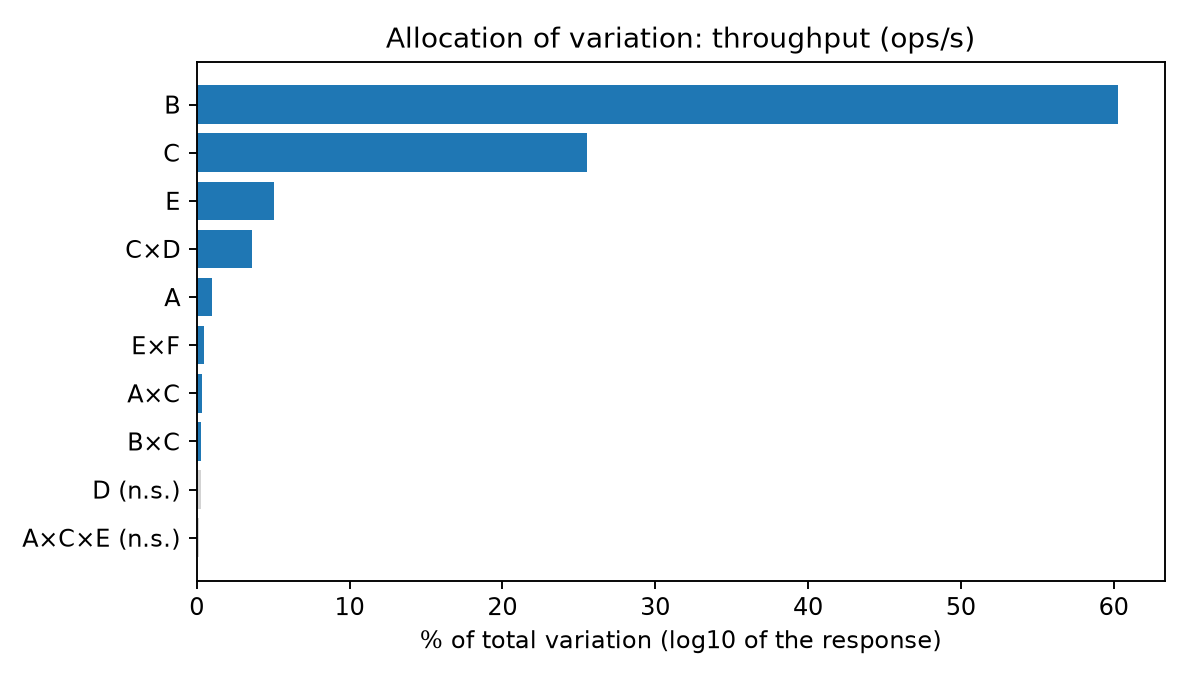
\includegraphics[height=3.9cm]{pareto_throughput_ops_sec.png}
  \hfill
  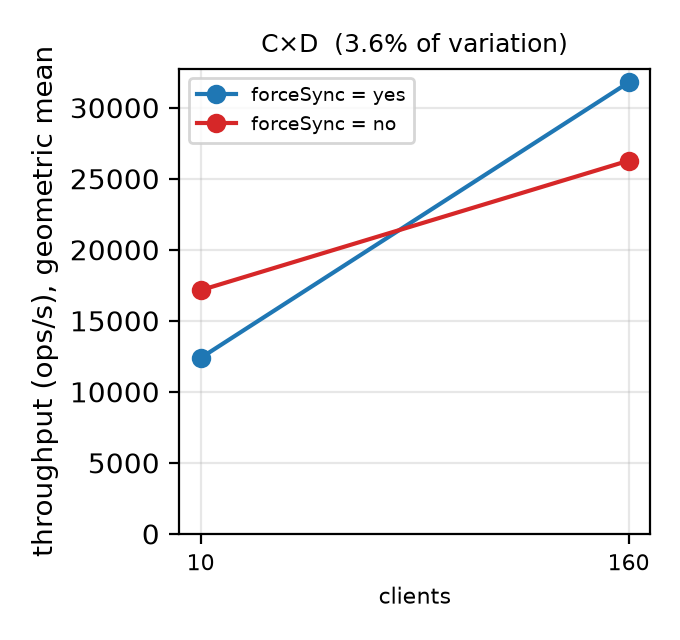
\includegraphics[height=3.9cm]{interactions_throughput_ops_sec.png}
  \caption{Left: share of the variation of $\log_{10}$ throughput per effect (ten largest). Right: clients $\times$
    \texttt{forceSync}.}
  \label{fig:pareto}
\end{figure}

\subsection{USL curve}
\label{sec:usl}

We measured one configuration (3 servers, 30\% writes, 128\,B) at 13 client counts from 1 to 160, with three replicates
per level in random order. In the notation of the course,
\begin{equation}
  X(N)=\frac{\lambda N}{1+\sigma(N-1)+\kappa N(N-1)},
\end{equation}
where $\lambda$ is the throughput of one client, $\sigma$ the contention (serial) coefficient and $\kappa$ the crosstalk
(coherency) coefficient. The fit minimizes relative error, so that 3\% counts the same at 600 and at 6{,}000 ops/s. The
intervals come from a bootstrap over the replicates. We compare the full model with the contention-only (Amdahl) model by
AIC and an F-test, and validate it by fitting $N\le64$ and predicting the three highest loads. The number of servers is not
varied here; its effect is factor A above.

\begin{figure}[t]
  \centering
  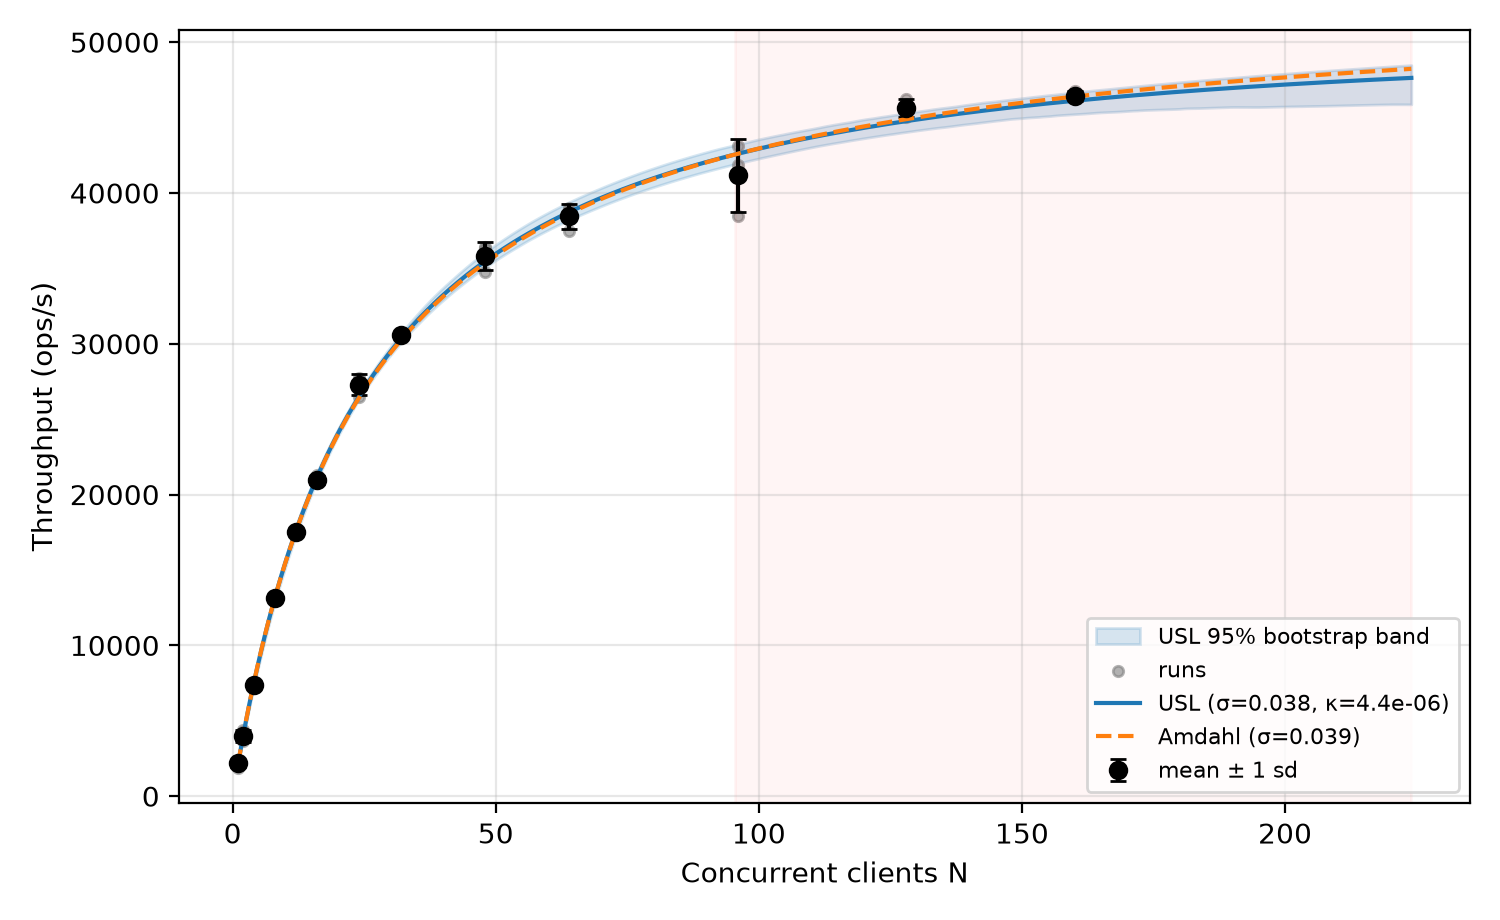
\includegraphics[width=0.85\textwidth]{usl_single_fit.png}
  \caption{Throughput against clients: runs, mean $\pm$ one standard deviation, the USL fit with its 95\% bootstrap band
    and the Amdahl model. The shaded region was held out for validation.}
  \label{fig:usl}
\end{figure}

Throughput rises from 2{,}165 ops/s with one client to 46{,}436 ops/s with 160 (Fig.~\ref{fig:usl}); the client stayed
below 28\% CPU. The fit gives $\lambda=2{,}082$ ops/s (95\% interval 1{,}996--2{,}169) and $\sigma=0.0385$
(0.0345--0.0414). The crosstalk term is not supported: the Amdahl model has the lower AIC ($-241.4$ against $-239.5$),
the F-test gives $p=0.72$, and 37\% of the bootstrap fits put $\kappa$ at zero. We therefore use the Amdahl fit
($\lambda=2{,}088$, $\sigma=0.039$) and claim no retrograde region within 160 clients. It bounds throughput by
$\lambda/\sigma\approx53{,}500$ ops/s; at 160 clients the system delivers 87\% of that. The efficiency $X(N)/(N\lambda)$
falls to 0.74 at 10 clients and 0.13 at 160. Fitted on $N\le64$ only, the model predicts the throughput at 96, 128 and
160 clients within 1.9--5.1\%.

\paragraph{Response time.} Combining the Amdahl fit with Little's law for a closed loop without think time gives
\begin{equation}
  R(N)=\frac{N}{X(N)}=\frac{1+\sigma(N-1)}{\lambda},
\end{equation}
a floor of $1/\lambda=0.48$\,ms plus $\sigma/\lambda=19\,\mu$s for every added client: once the system saturates, each new
client only adds waiting time. Table~\ref{tab:latency} compares it with the measured mean $N/X$ and with the median and
95th percentile recorded by the client. The model and $N/X$ agree within 3.7\% at every level, which mostly restates the
quality of the throughput fit. The mean lies between the measured median and 95th percentile at every level, as expected
for a right-skewed distribution.

\begin{table}[t]
  \centering
  \caption{Mean response time from the Amdahl fit and Little's law, against measured latencies (all operations).}
  \label{tab:latency}
  \scriptsize
  \begin{tabular}{@{}lrrrrrr@{}}
\toprule
Clients $N$ & 1 & 8 & 32 & 64 & 128 & 160 \\
\midrule
$R(N)$ predicted (ms) & 0.48 & 0.61 & 1.06 & 1.66 & 2.85 & 3.45 \\
$N/X$ measured (ms) & 0.46 & 0.61 & 1.05 & 1.66 & 2.81 & 3.45 \\
median (ms) & 0.22 & 0.28 & 0.49 & 0.87 & 1.64 & 2.42 \\
95th perc. (ms) & 1.15 & 1.79 & 2.95 & 4.48 & 7.50 & 8.75 \\
\bottomrule
\end{tabular}

\end{table}

\paragraph{Per-stage times.} Table~\ref{tab:stages} gives ZooKeeper's timers on the leader at four of the 13 levels
(all levels: Fig.~\ref{fig:stages}). From 1 to 160 clients the server-side write latency grows from 0.87 to 5.57\,ms. The
intervals overlap and do not add up: the time to quorum acknowledgment starts when the proposal is created and includes
the leader's own log sync and the followers' round trip. In absolute terms the time to quorum acknowledgment grows most
($+2.07$\,ms). The queue in front of request preparation grows most in relative terms, from 0.02 to 1.37\,ms, and most of
that growth happens beyond 64 clients. The log-sync queue, in contrast, levels off at about 0.7\,ms, because the batch
grows from 1 to 17.6 requests per \texttt{fsync}.

\begin{table}[t]
  \centering
  \caption{Leader per-stage times (ms, mean of the replicates) and requests per \texttt{fsync}. 1\,ms timer resolution.}
  \label{tab:stages}
  \scriptsize
  \begin{tabular}{@{}lrrrr@{}}
\toprule
Leader, mean per run & $N=1$ & $N=16$ & $N=64$ & $N=160$ \\
\midrule
prep queue (zxid) (ms) & 0.02 & 0.05 & 0.35 & 1.37 \\
sync queue (ms) & 0.03 & 0.43 & 0.66 & 0.76 \\
sync queue + flush (ms) & 0.55 & 1.08 & 1.86 & 2.14 \\
fsync (ms) & 0.06 & 0.22 & 0.69 & 0.75 \\
until quorum ACK (ms) & 0.72 & 1.34 & 2.26 & 2.79 \\
server-side write latency (ms) & 0.87 & 1.61 & 3.26 & 5.57 \\
requests per fsync & 1.0 & 4.1 & 13.0 & 17.6 \\
\bottomrule
\end{tabular}

\end{table}

\subsection{eBPF probes}
\label{sec:ebpf}

Four probes are our own bpftrace programs~\cite{gregg_bpf} and one is bcc's \texttt{runqlat}:
\begin{itemize}
  \item \texttt{fsync} latency: syscall tracepoints of \texttt{fsync}/\texttt{fdatasync}, ZooKeeper's JVM only;
  \item block I/O latency per disk: \texttt{block\_rq\_issue} to \texttt{block\_rq\_complete} (bcc's
    \texttt{biolatency} uses a kprobe that is not traceable on kernel 6.1);
  \item run-queue latency of the JVM's threads (\texttt{runqlat});
  \item TCP retransmissions and resets (\texttt{tcp} tracepoints);
  \item CPU per thread: a 99\,Hz \texttt{profile} probe keyed by thread name. ZooKeeper names the thread of each stage
    and the JVM passes the names to Linux, so this gives the CPU of each stage.
\end{itemize}
They ran on the leader in separate runs (3 servers, 80 clients, 50\% writes) at both levels of \texttt{forceSync} and log
disk. Each probed run is preceded by a discarded warm-up run and placed between two identical runs without probes.
Tables~\ref{tab:ebpf} and~\ref{tab:ebpfzk} give the results.

\begin{table}[t]
  \centering
  \caption{Kernel view of the leader. Percentiles are upper bounds of log$_2$ histogram buckets.}
  \label{tab:ebpf}
  \scriptsize
  \setlength{\tabcolsep}{3pt}
  \resizebox{\linewidth}{!}{\begin{tabular}{@{}lrrrrrr@{}}
\toprule
Configuration & fsync calls & fsync mean ($\mu$s) & fsync p99 ($\mu$s) & log disk p99 ($\mu$s) & run queue p99 ($\mu$s) & TCP retr. \\
\midrule
fsync off, pd-balanced & 0 & -- & -- & 16384 & 511 & 0 \\
fsync off, pd-ssd & 0 & -- & -- & 16384 & 511 & 0 \\
fsync on, pd-balanced & 21393 & 1064 & 2048 & 1024 & 511 & 0 \\
fsync on, pd-ssd & 23120 & 986 & 2048 & 512 & 511 & 0 \\
\bottomrule
\end{tabular}
}
\end{table}

\begin{table}[t]
  \centering
  \caption{The probed runs seen by the client and by ZooKeeper (top) and the leader's CPU per thread, in cores (bottom).}
  \label{tab:ebpfzk}
  \scriptsize
  \setlength{\tabcolsep}{3pt}
  \resizebox{\linewidth}{!}{\begin{tabular}{@{}lrrrrrr@{}}
\toprule
Configuration & ops/s & no probes & overhead (\%) & req./fsync & ZK fsync (ms) & to quorum ACK (ms) \\
\midrule
fsync off, pd-balanced & 29276 & 28795 & -1.7 & 1.9 & -- & 1.14 \\
fsync off, pd-ssd & 28739 & 24992 & -15.0 & 1.8 & -- & 1.16 \\
fsync on, pd-balanced & 26622 & 28731 & 7.3 & 17.4 & 0.77 & 2.56 \\
fsync on, pd-ssd & 26674 & 27301 & 2.3 & 16.0 & 0.70 & 2.52 \\
\bottomrule
\end{tabular}
}\\[4pt]
  \resizebox{\linewidth}{!}{\begin{tabular}{@{}lrrrr@{}}
\toprule
CPU cores used by & fsync off, pd-balanced & fsync off, pd-ssd & fsync on, pd-balanced & fsync on, pd-ssd \\
\midrule
replication to followers & 0.67 & 0.67 & 0.55 & 0.59 \\
client connections (I/O) & 0.40 & 0.38 & 0.40 & 0.39 \\
PrepRequestProcessor (zxid) & 0.20 & 0.21 & 0.25 & 0.25 \\
CommitProcessor & 0.19 & 0.18 & 0.17 & 0.16 \\
SyncRequestProcessor (log, fsync) & 0.10 & 0.09 & 0.10 & 0.11 \\
commit workers (apply, reply) & 0.06 & 0.05 & 0.06 & 0.06 \\
JIT compiler & 0.05 & 0.06 & 0.03 & 0.03 \\
whole JVM & 1.73 & 1.70 & 1.61 & 1.62 \\
\bottomrule
\end{tabular}
}
\end{table}

\paragraph{The \texttt{fsync} and the disk.} With \texttt{forceSync=no} the probe sees no \texttt{fsync}, which confirms that
factor D was applied. With it, an \texttt{fsync} takes 1.0\,ms on average on both disks. Its histogram has two modes: 21--27\%
of the calls take 256--512\,$\mu$s and 68--75\% take 1--2\,ms. The block-I/O histograms of the two disks are almost the
same, with 85--88\% of the requests in the 256--512\,$\mu$s bucket. The p99 of pd-ssd falls one bucket lower only because
slightly fewer requests cross 512\,$\mu$s, so we cannot call one disk faster than the other, and that agrees with F having
no effect. There are about 2.7 block requests per \texttt{fsync}. Our reading is that an ext4 \texttt{fsync} that must also
commit the journal waits for several device round trips in sequence (data, journal, cache flush), which would explain both
the 1--2\,ms mode and why an \texttt{fsync} costs more than the device's p99. We did not trace the journal to confirm it.
Without \texttt{fsync} the log disk sees only about 390 requests in 45\,s, most of them taking 1--8\,ms. These are background
write-backs of dirty pages, merged into large requests, and no request waits for them.

\paragraph{CPU, scheduler and network.} The leader's JVM uses 1.6--1.7 of its two vCPUs. The largest shares are
replication to the followers (0.55--0.67 cores) and client connections (0.4); request preparation uses 0.20--0.25 and the
log-sync thread 0.1. The run-queue p99 is below 0.5\,ms and there are no retransmissions.

\paragraph{What the probe runs cannot show.} The two runs without probes around each probed run differed by 6\% to 43\%,
and the apparent probe overhead ranges from $-15\%$ to $+7\%$. The spread in these runs is larger than any overhead we
could detect, so we cannot quantify the overhead below about 15\%. It is also larger than the difference between the
configurations: with probes, the runs without \texttt{fsync} are 9\% faster, while the unprobed runs show them 4\% slower.
We therefore draw no conclusion on throughput at 80 clients from these runs. We use them only for quantities that the
probes measure directly (call counts, histograms, CPU shares) and that changed little between runs.

\section{Discussion: What Limits Scalability}
\label{sec:discussion}

Table~\ref{tab:limits} maps each term of the USL, and the number of servers, to the parts of the pipeline it can come
from, and lists the evidence we have and what could be done about it.

\begin{table}[t]
  \centering
  \caption{USL terms and number of servers: candidate stages, evidence and mitigations.}
  \label{tab:limits}
  \scriptsize
  \begin{tabularx}{\linewidth}{@{}>{\raggedright\arraybackslash}p{1.1cm}*{3}{>{\raggedright\arraybackslash}X}@{}}
    \toprule
    Term & Candidate stages & Evidence & Mitigation \\
    \midrule
    $\sigma$ & Work the leader does for every write: ordering, replication, log sync; its CPU
      & $\sigma=0.039$; no thread near a full core; JVM at 1.6--1.7 of 2 cores; D and F do not raise throughput at saturation
      & More CPU for the leader; \texttt{leaderServes=no}; batched writes (multi-operations) \\
    $\kappa$ & Interference growing with pairs of clients (per-session state, GC, commit waits on reads)
      & Not supported ($p=0.72$; 37\% of bootstrap fits at zero)
      & --- \\
    $\lambda$ & Cost of one request alone: round trips, serialization, payload, one \texttt{fsync}
      & $\lambda=2{,}082$ ops/s (0.48\,ms per request); 4\,KiB payloads $\times0.74$; quorum ACK 0.72\,ms at $N=1$
      & Asynchronous clients; smaller payloads \\
    Servers (A) & Proposals to more followers vs.\ fewer sessions on the leader
      & $\times1.14$, mostly at 160 clients; same at both write ratios; no retransmissions
      & Observers for reads; \texttt{leaderServes=no} \\
    \bottomrule
  \end{tabularx}
\end{table}

\paragraph{Contention ($\sigma$).} The curve has one dominant limit, contention, and the disk does not cause it. An
\texttt{fsync} costs about 1\,ms on either disk, group commit spreads it over up to 17 requests at high load, and neither
D nor F raises throughput at saturation. Where the contention does come from is less clear. In the probed runs no
single thread is near a full core: the request-preparation thread uses a quarter of one and the log-sync thread a
tenth. So it is not one serial stage running out of CPU. What is close to its limit is the leader's CPU as a whole, at
1.6--1.7 of two cores, and most of it goes to replication and client connections. Run-queue waits stay short, so the
leader is not starved of CPU on each wake-up; but every write adds work to the same two cores, and the prep queue, which
grows fastest at high load, is where requests wait for that work to drain. Two caveats apply. The probes measured a
different configuration from the USL curve (80 clients and 50\% writes against 30\% writes), and the stage timers overlap.
We read $\sigma$ as the saturation of the leader's shared resources, mainly its CPU, under the per-write work of Zab.
Three results support this reading: five servers help most at 160 clients, where they take sessions off the leader;
turning \texttt{fsync} off hurts only at saturation; and the efficiency falls steadily from the lowest loads. A direct test
would repeat the sweep with a larger leader machine or with \texttt{leaderServes=no}; we did not run it.

\paragraph{Mitigations.} If $\sigma$ is the leader's CPU, the useful changes relieve the leader: giving it more CPU,
configuring it not to accept clients (\texttt{leaderServes=no})~\cite{zookeeper_admin}, adding observers so reads do not
need more voting servers, or batching writes in multi-operations so that the per-request replication work is spread the
way group commit spreads the \texttt{fsync}. A faster log disk would not help, and turning \texttt{fsync} off costs
throughput at high load as well as durability.

\section{Conclusion}

The workload decides ZooKeeper's throughput more than the configuration does: the share of writes explains 60\% of its
variation and the load 26\%, while the log disk explains nothing and \texttt{fsync} matters only through its interaction
with load. For the write tail latency the load explains 94\%. One replicated curve is described by contention alone
($\sigma=0.039$, $\lambda=2{,}082$ ops/s), levels off towards about 53{,}500 ops/s and is predicted within 5\% from the
lower half of the loads. The \texttt{fsync} costs about 1\,ms on both disks and group commit spreads it over up to 17
requests, so the disk does not limit scalability; our measurements point to the leader's CPU but do not prove it. The
Stage I artifact also taught us to validate the load generator before interpreting its numbers.

\emph{Limitations.} One zone; virtual machines with noisy neighbours (replicates differ by about 11\%); a 2-vCPU leader,
which makes CPU an early limit; disk results tied to 20\,GB disks on small machines; one USL configuration; probes in a
different configuration from the curve, with run-to-run noise larger than the probe overhead; a workload without creates,
deletes, watches or multi-operations. The next experiments are the USL sweep with a larger leader and with
\texttt{leaderServes=no}, and the same sweep with observers.

\begin{thebibliography}{11}

\bibitem{hunt_zookeeper}
P.~Hunt, M.~Konar, F.~P. Junqueira, and B.~Reed.
\newblock ZooKeeper: Wait-free coordination for Internet-scale systems.
\newblock In \emph{USENIX Annual Technical Conference}, 2010.

\bibitem{apache_zookeeper_overview}
Apache Software Foundation.
\newblock ZooKeeper: A Distributed Coordination Service for Distributed Applications.
\newblock ZooKeeper 3.9.6 documentation, 2024.
\newblock \url{https://zookeeper.apache.org/doc/r3.9.6/zookeeperOver.html}.

\bibitem{zab_junqueira}
F.~P. Junqueira, B.~C. Reed, and M.~Serafini.
\newblock Zab: High-performance broadcast for primary-backup systems.
\newblock In \emph{IEEE/IFIP International Conference on Dependable Systems and Networks (DSN)}, 2011.

\bibitem{gunther_usl_dsconf}
Distributed Systems Conference.
\newblock Applying The Universal Scalability Law to Distributed Systems by Dr. Neil J. Gunther.
\newblock DSConf 2019, March 16, 2019.
\newblock \url{https://www.youtube.com/watch?v=cuieNj3NrZ8}.

\bibitem{gunther_book}
N.~J. Gunther.
\newblock \emph{Guerrilla Capacity Planning}.
\newblock Springer, 2007.

\bibitem{zookeeper_admin}
Apache Software Foundation.
\newblock ZooKeeper Administrator's Guide.
\newblock ZooKeeper 3.9.3 documentation.
\newblock \url{https://zookeeper.apache.org/doc/r3.9.3/zookeeperAdmin.html}.

\bibitem{mit_6824_zookeeper}
MIT 6.824: Distributed Systems.
\newblock ZooKeeper.
\newblock Lecture 8, Spring 2020.
\newblock \url{https://www.youtube.com/watch?v=pbmyrNjzdDk}.

\bibitem{jain_book}
R.~Jain.
\newblock \emph{The Art of Computer Systems Performance Analysis}.
\newblock Wiley, 1991.

\bibitem{gregg_bpf}
B.~Gregg.
\newblock \emph{BPF Performance Tools}.
\newblock Addison-Wesley, 2019.

\bibitem{ycsb}
B.~F. Cooper, A.~Silberstein, E.~Tam, R.~Ramakrishnan, and R.~Sears.
\newblock Benchmarking cloud serving systems with YCSB.
\newblock In \emph{ACM Symposium on Cloud Computing (SoCC)}, 2010.

\bibitem{pumba}
A.~Ledenev.
\newblock Pumba: chaos testing and network emulation for Docker containers.
\newblock \url{https://github.com/alexei-led/pumba}.

\end{thebibliography}

\appendix

\section{Stage I experiments not repeated in Stage II}
\label{app:stage1}

These runs were made on the Stage I laptop with the servers in Docker containers, one run per cell and no confidence
intervals. They come from a different testbed and are kept only as context.

\paragraph{YCSB.} We ran YCSB~\cite{ycsb} with its ZooKeeper binding on 3 servers (Table~\ref{tab:ycsb}). At 16 threads the
read-heavy workloads B and C reach about 6.7 times the throughput of the 50/50 workload A, and in A an update takes
3--4.5 times as long as a read on average (3{,}713 against 1{,}078\,$\mu$s). B and C peak at 16 threads. Workload A jumps
from 1{,}723 to 5{,}964 ops/s between 16 and 32 threads; with a single run per cell we cannot tell whether this is a real
effect or noise, warm-up or garbage collection.

\begin{table}[h]
  \centering
  \caption{YCSB throughput (ops/s), Stage I laptop, 3 servers, one run per cell.}
  \label{tab:ycsb}
  \scriptsize
  \begin{tabular}{@{}lrrrr@{}}
    \toprule
    Workload & 1 thread & 4 & 16 & 32 \\
    \midrule
    A (50/50 read/update) & 790  & 1316 & 1723  & 5964 \\
    B (95/5)              & 3544 & 6927 & 11436 & 8080 \\
    C (100\% read)        & 4538 & 9074 & 11913 & 8900 \\
    \bottomrule
  \end{tabular}
\end{table}

\paragraph{Leader failover.} During a continuous benchmark on 3 servers we found the leader with \texttt{stat} and killed
its container. The two survivors kept a majority and continued, and ZooKeeper logged an election of 211\,ms (216 and
235\,ms in a repetition). This is ZooKeeper's measurement of the election only; we did not measure the outage seen by
clients.

\paragraph{Network delay.} We added 20$\pm$2\,ms to the egress of every server container with Pumba~\cite{pumba} (which
drives \texttt{tc netem} inside each container's network namespace) and repeated the sweep with the quiet client
(Table~\ref{tab:chaos}). Throughput per client stays at about 21.5 ops/s, one operation per 46.5\,ms, at every load: the
clients wait on the delay and the servers never saturate within 80 clients. The median read took 22.7\,ms (one delayed
hop) and the median write 106\,ms (about five: forward, proposal, acknowledgment, commit, reply), as
Fig.~\ref{fig:pipeline} predicts for a client attached to a follower. We did not fit the USL to these data.

\begin{table}[h]
  \centering
  \caption{Throughput (ops/s) with and without a 20\,ms egress delay, Stage I laptop, 3 servers, one run per cell.}
  \label{tab:chaos}
  \scriptsize
  \begin{tabular}{@{}lrrrrrr@{}}
    \toprule
    Clients & 1 & 5 & 10 & 20 & 40 & 80 \\
    \midrule
    No delay      & 2386 & 7016 & 11680 & 14832 & 16238 & 16255 \\
    20\,ms delay  & 20.6 & 108.9 & 216.7 & 434.6 & 865.5 & 1709 \\
    \bottomrule
  \end{tabular}
\end{table}

\section{Per-stage times at every load level}
\label{app:stages}

\begin{figure}[h]
  \centering
  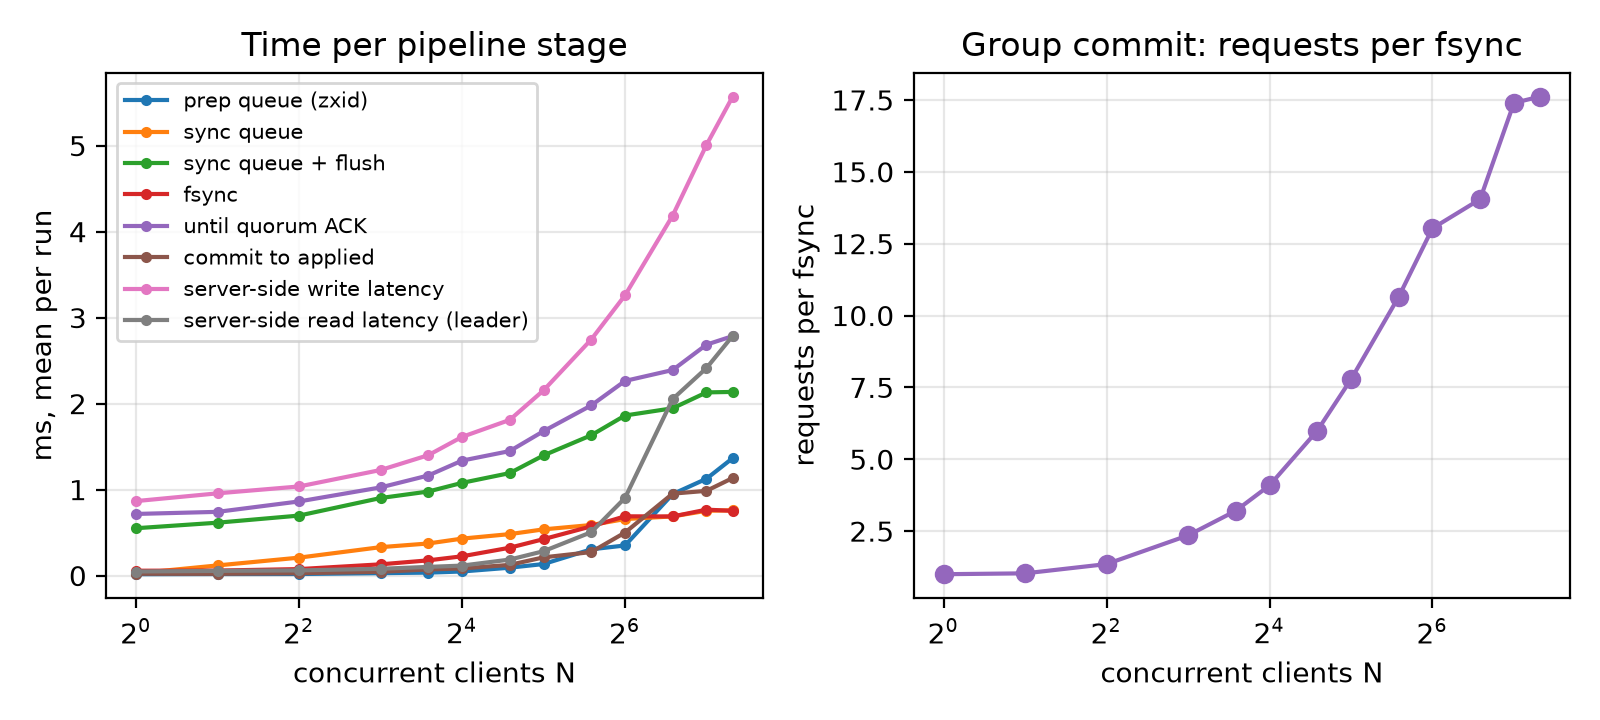
\includegraphics[width=\textwidth]{stage_breakdown.png}
  \caption{Leader per-stage times (left) and requests per \texttt{fsync} (right) at every level of the USL curve.}
  \label{fig:stages}
\end{figure}

\section{Model checks}
\label{app:residuals}

\begin{figure}[h]
  \centering
  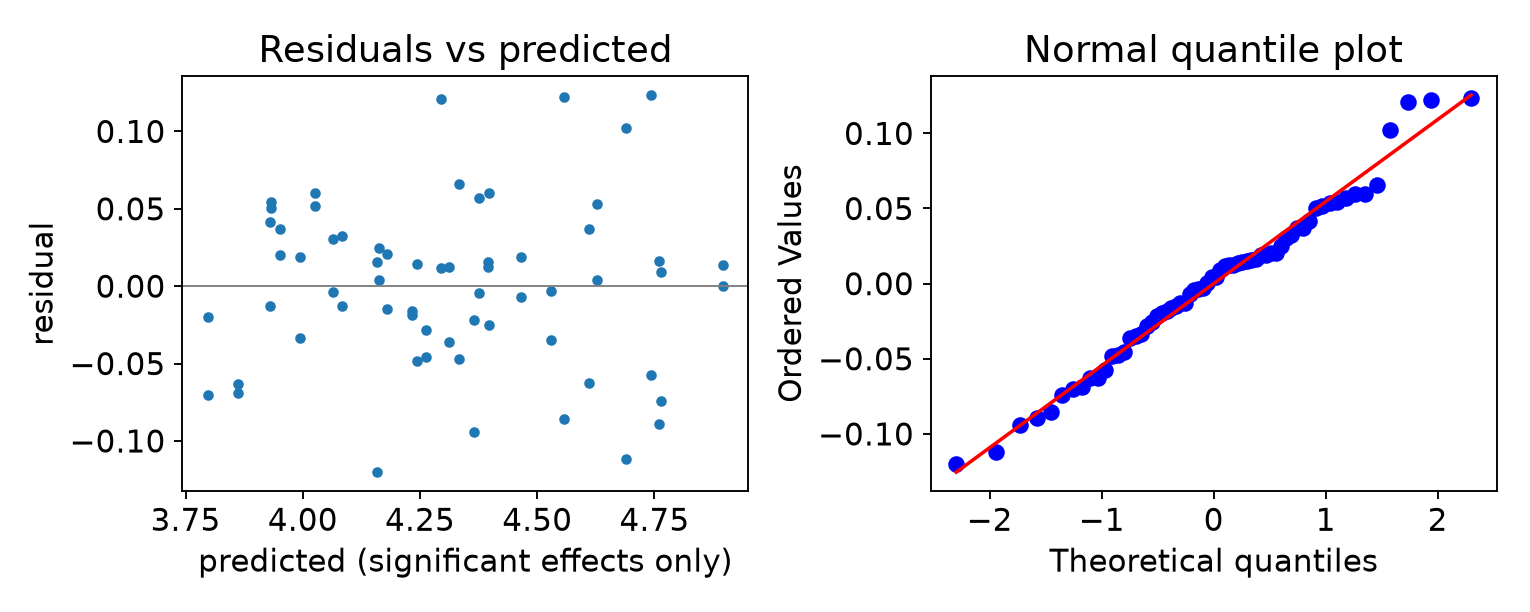
\includegraphics[width=0.9\textwidth]{residuals_throughput_ops_sec.png}\\
  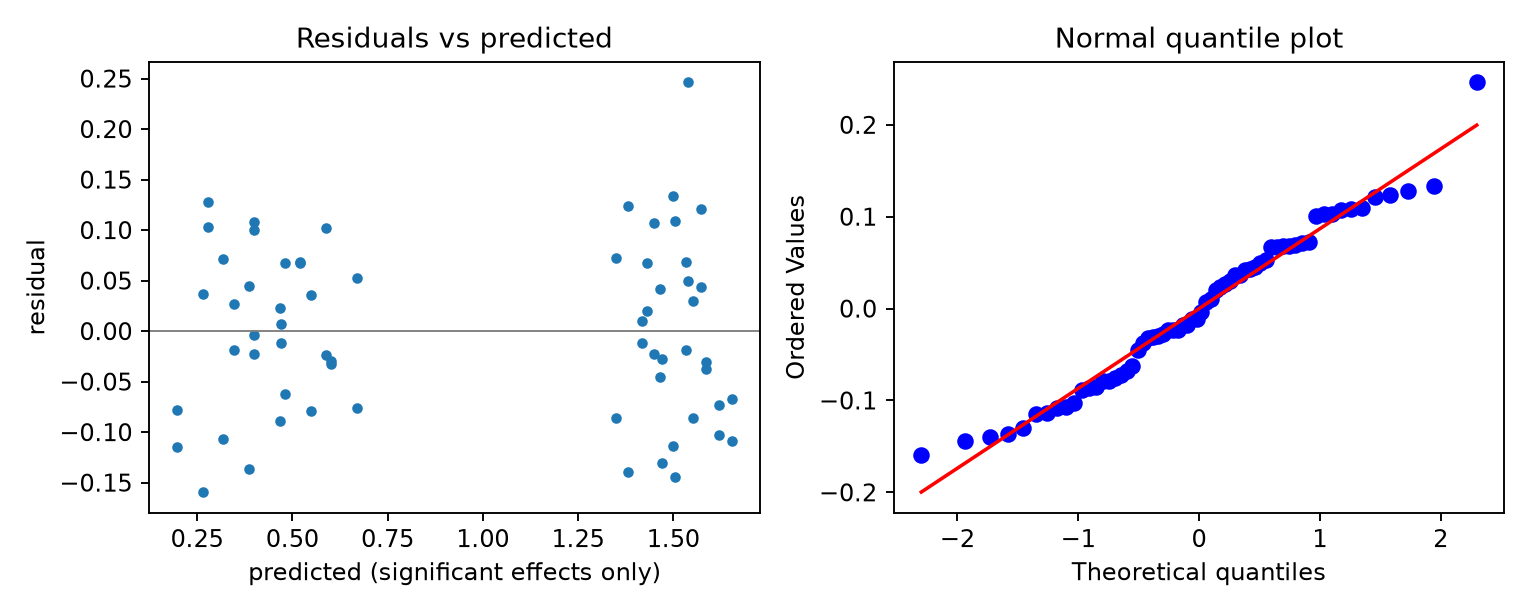
\includegraphics[width=0.9\textwidth]{residuals_write_p99_ms.png}
  \caption{Residuals of the $\log_{10}$ effects model against the predicted value (left) and normal quantile plots
    (right): throughput (top) and write p99 (bottom).}
  \label{fig:residuals}
\end{figure}

\end{document}
